\documentclass[tikz,border=1.35mm]{standalone}

% Plain quadrilateral face used in the FVMAdapt overview figures.
% Coordinates are in millimeters; y=-1mm keeps the SVG-style origin at top left.
\begin{document}
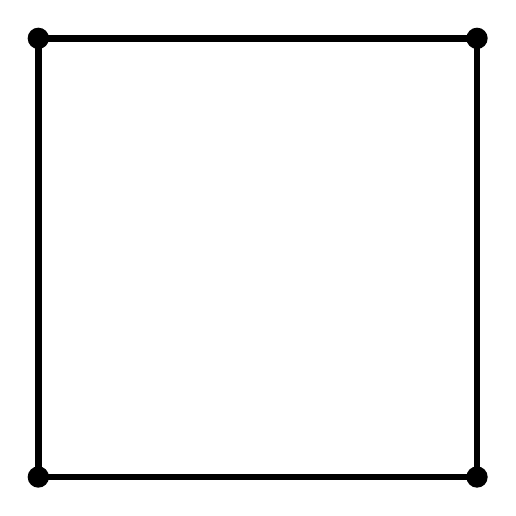
\begin{tikzpicture}[x=1mm,y=-1mm,line join=round]
  % Match the original artwork frame before the standalone border is applied.
  \useasboundingbox (0,0) rectangle (58.419,58.419);

  % Quadrilateral vertices, ordered around the face.
  \coordinate (v0) at (1.353,1.353);
  \coordinate (v1) at (57.067,1.353);
  \coordinate (v2) at (57.067,57.067);
  \coordinate (v3) at (1.353,57.067);

  % Draw edges first so vertex markers sit cleanly on top.
  \draw[line width=0.865mm] (v0) rectangle (v2);

  % Original vertices are black.
  \fill[black] (v0) circle[radius=1.353mm];
  \fill[black] (v1) circle[radius=1.353mm];
  \fill[black] (v2) circle[radius=1.353mm];
  \fill[black] (v3) circle[radius=1.353mm];
\end{tikzpicture}
\end{document}
